\chapter{Data}

\begin{figure}[H]
    \centering
    \begin{tabular}{| l | c c c c |} 
        \hline
        \textbf{Dataset} & \textbf{\# Sequences} & \textbf{Multi-person} & \textbf{Text descriptions} & \textbf{Scene object} \\ \hline
        HumanML3D & 14,616 & \xmark & \cmark (44,970) & \xmark \\
        InterHuman & 7,779 & \cmark (exactly 2) & \cmark (16,756) & \xmark \\
        Teton & 27,656 & \cmark & \xmark & \cmark \\
        \hline
    \end{tabular}
    \caption{Overview of different dataset properties.}
\end{figure}


\section{HumanML3D}
The HumanML3D dataset combines the HumanAct12 and AMASS datasets, integrating human motion captured using advanced motion capturing systems and converting the data to a unified parameterization. It covers a broad range of daily human activities, providing 14,616 motions in total, accompanied by 44,970 single-sentence descriptions. Each motion clip includes 3-4 descriptions, and the entire dataset amounts to 28.59 hours of recorded motion. Additionally, the data is augmented by mirroring all motions, with corresponding adjustments to descriptions, such as changing “clockwise” to “counterclockwise.”


\section{InterHuman}
The InterHuman dataset is a comprehensive, large-scale 3D dataset designed to capture human interactive motions involving two individuals. It includes approximately 107 million frames detailing a wide range of human interactions, from professional activities to daily social behaviors. Each motion sequence is paired with natural language annotations, totaling 23,337 descriptions, which provide context and detail for the captured interactions, enhancing the dataset’s utility for training and evaluating models.

% 7779 sequences resulting in 6.56h 

\section{Teton (raw) dataset}
% \begin{figure}[H]
%     \centering
%     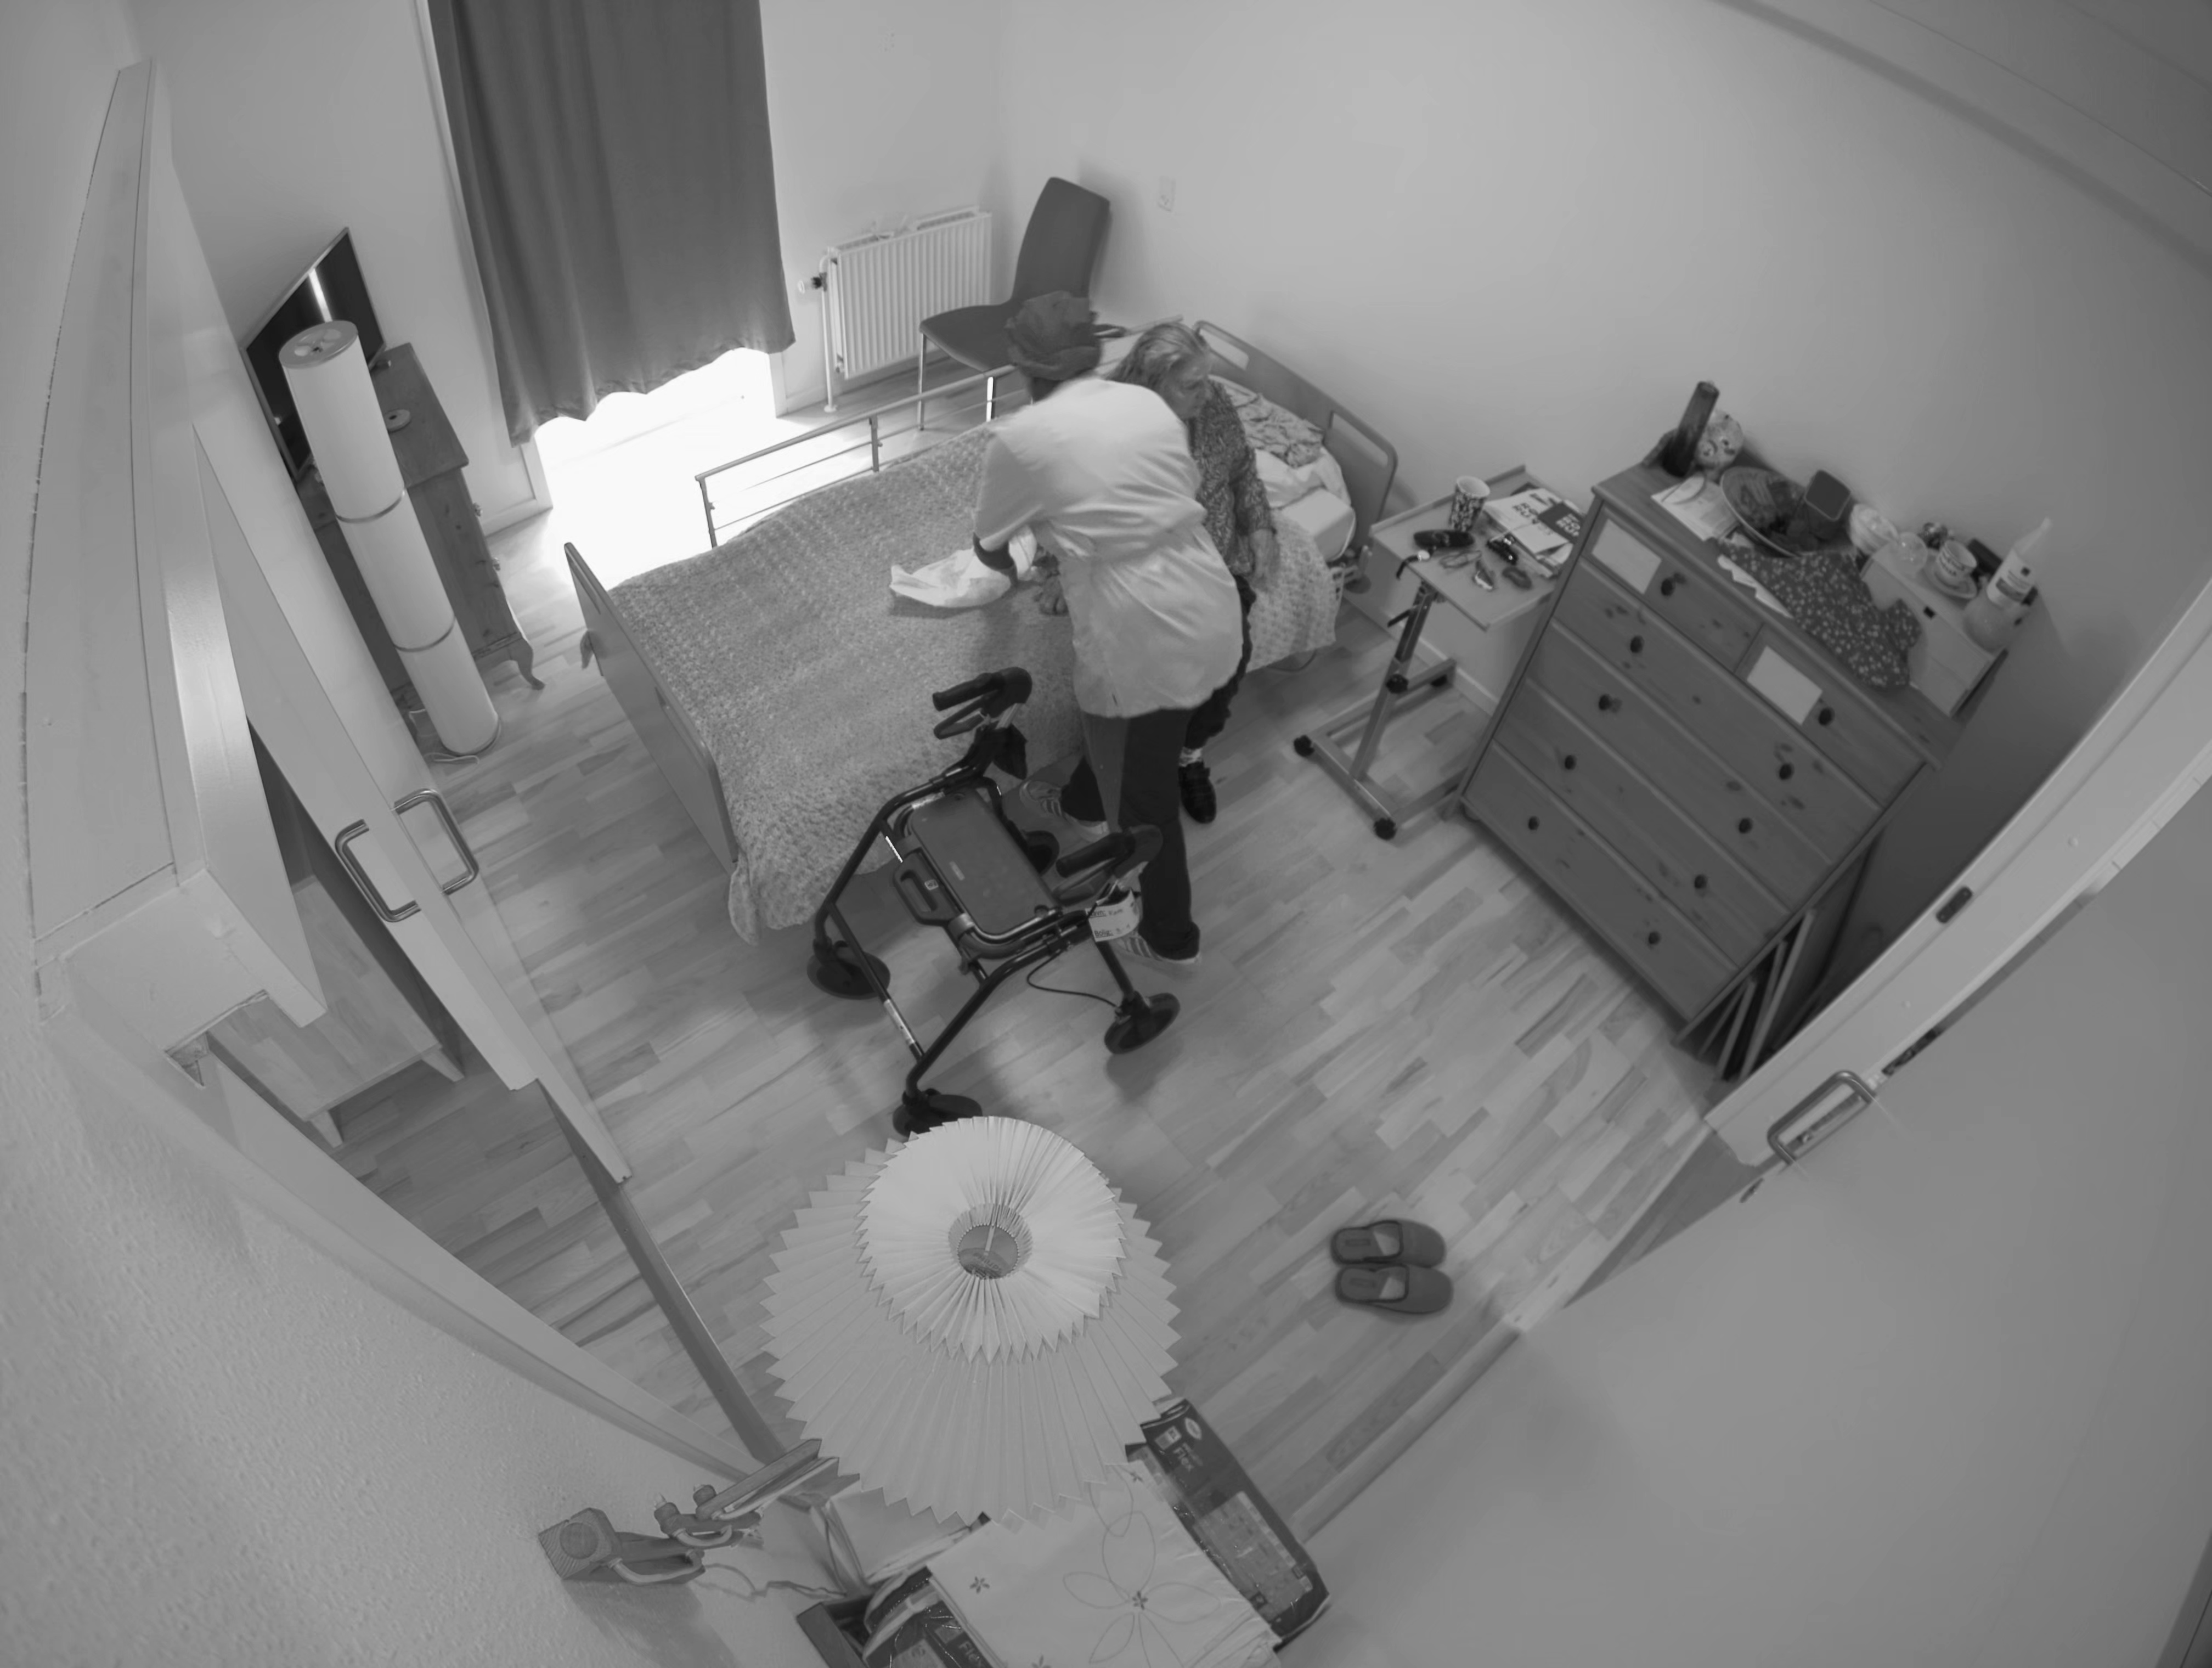
\includegraphics[width=0.6\linewidth]{figures/example-frame.png}
%     \caption{Examples from the Teton dataset}
% \end{figure}
The Teton dataset contains approximately 50,000 image sequences hierarchically organized by hospital/carehome site, room and timestamp. Each sequence consists of 100 frames recorded at approximately 10 frames per second, resulting in a sequence duration of about 10 seconds and totaling roughly 140 hours of data. 

Each person in the frame has been manually annotated with their class (person, staff, patient), center point, bounding box, keypoints and current action (e.g., "laying in bed", "standing on floor"). Using an image similarity threshold, the 100 frames are reduced to a smaller set of key frames. Each key frame is annotated with segmentation masks for people in the frame as well as the floor, walls and furniture (e.g., beds, sofas and chairs).

As the dataset is inheriently two dimensional and does not contain 3D annotations such as poses or depth maps, we instead rely on pseudo-ground truth data derived from off-the-shelf models. In the case of human poses the HMR2.0 model by \cite{goel2023humans} is initially run on the image sequences to predict a set of poses. Poses with high reprojection error are filtered out, and the remaining poses with low reprojection error are used as pseudo-ground truth. 

For reconstructing depth maps the monocular metric depth estimation model, Depth Anything by \cite{depthanything}, trained on the indoor NYUv2 dataset (\cite{SilbermanECCV12}), is applied to the set of key frames.



% These filtered poses are then used to train Teton's in-house model, which is based on a YOLOv7 backbone. Once trained, the Teton model is applied again to the entire dataset to extract per-frame SMPL poses.


% The dataset is structured by different levels. Top level is the department, next level is device/particular room, then date and time follows.
